\subsection{Geometry}
\begin{itemize}
   \item latest geometry in Figure \ref{fig:init}
   \item corresponding electric field for $p=3$, $n_\mathrm{sub}=16$,  $V_\mathrm{el}=-300\ \mathrm{kV}$ and $V_\mathrm{ar}=1\ \mathrm{kV}$
   \item (patches $32 \dots 35$ are not entirely correct, missing the correct high voltage adapter)
\end{itemize}

\begin{center}
\begin{figure}[H]
   \begin{subfigure}{0.45\textwidth}
      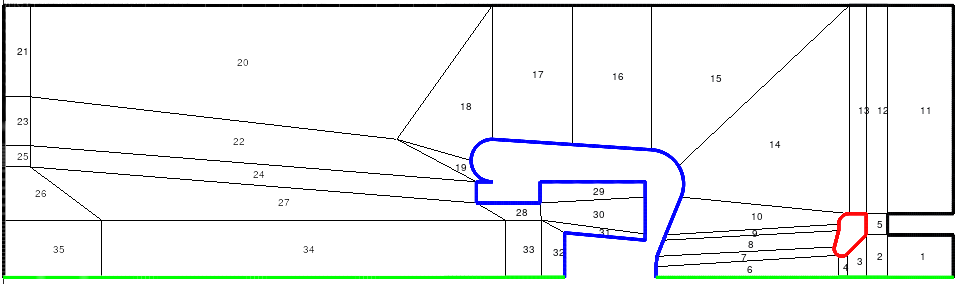
\includegraphics[width=\textwidth]{fig/geometry_v6}
   \end{subfigure}
   \begin{subfigure}{0.45\textwidth}
      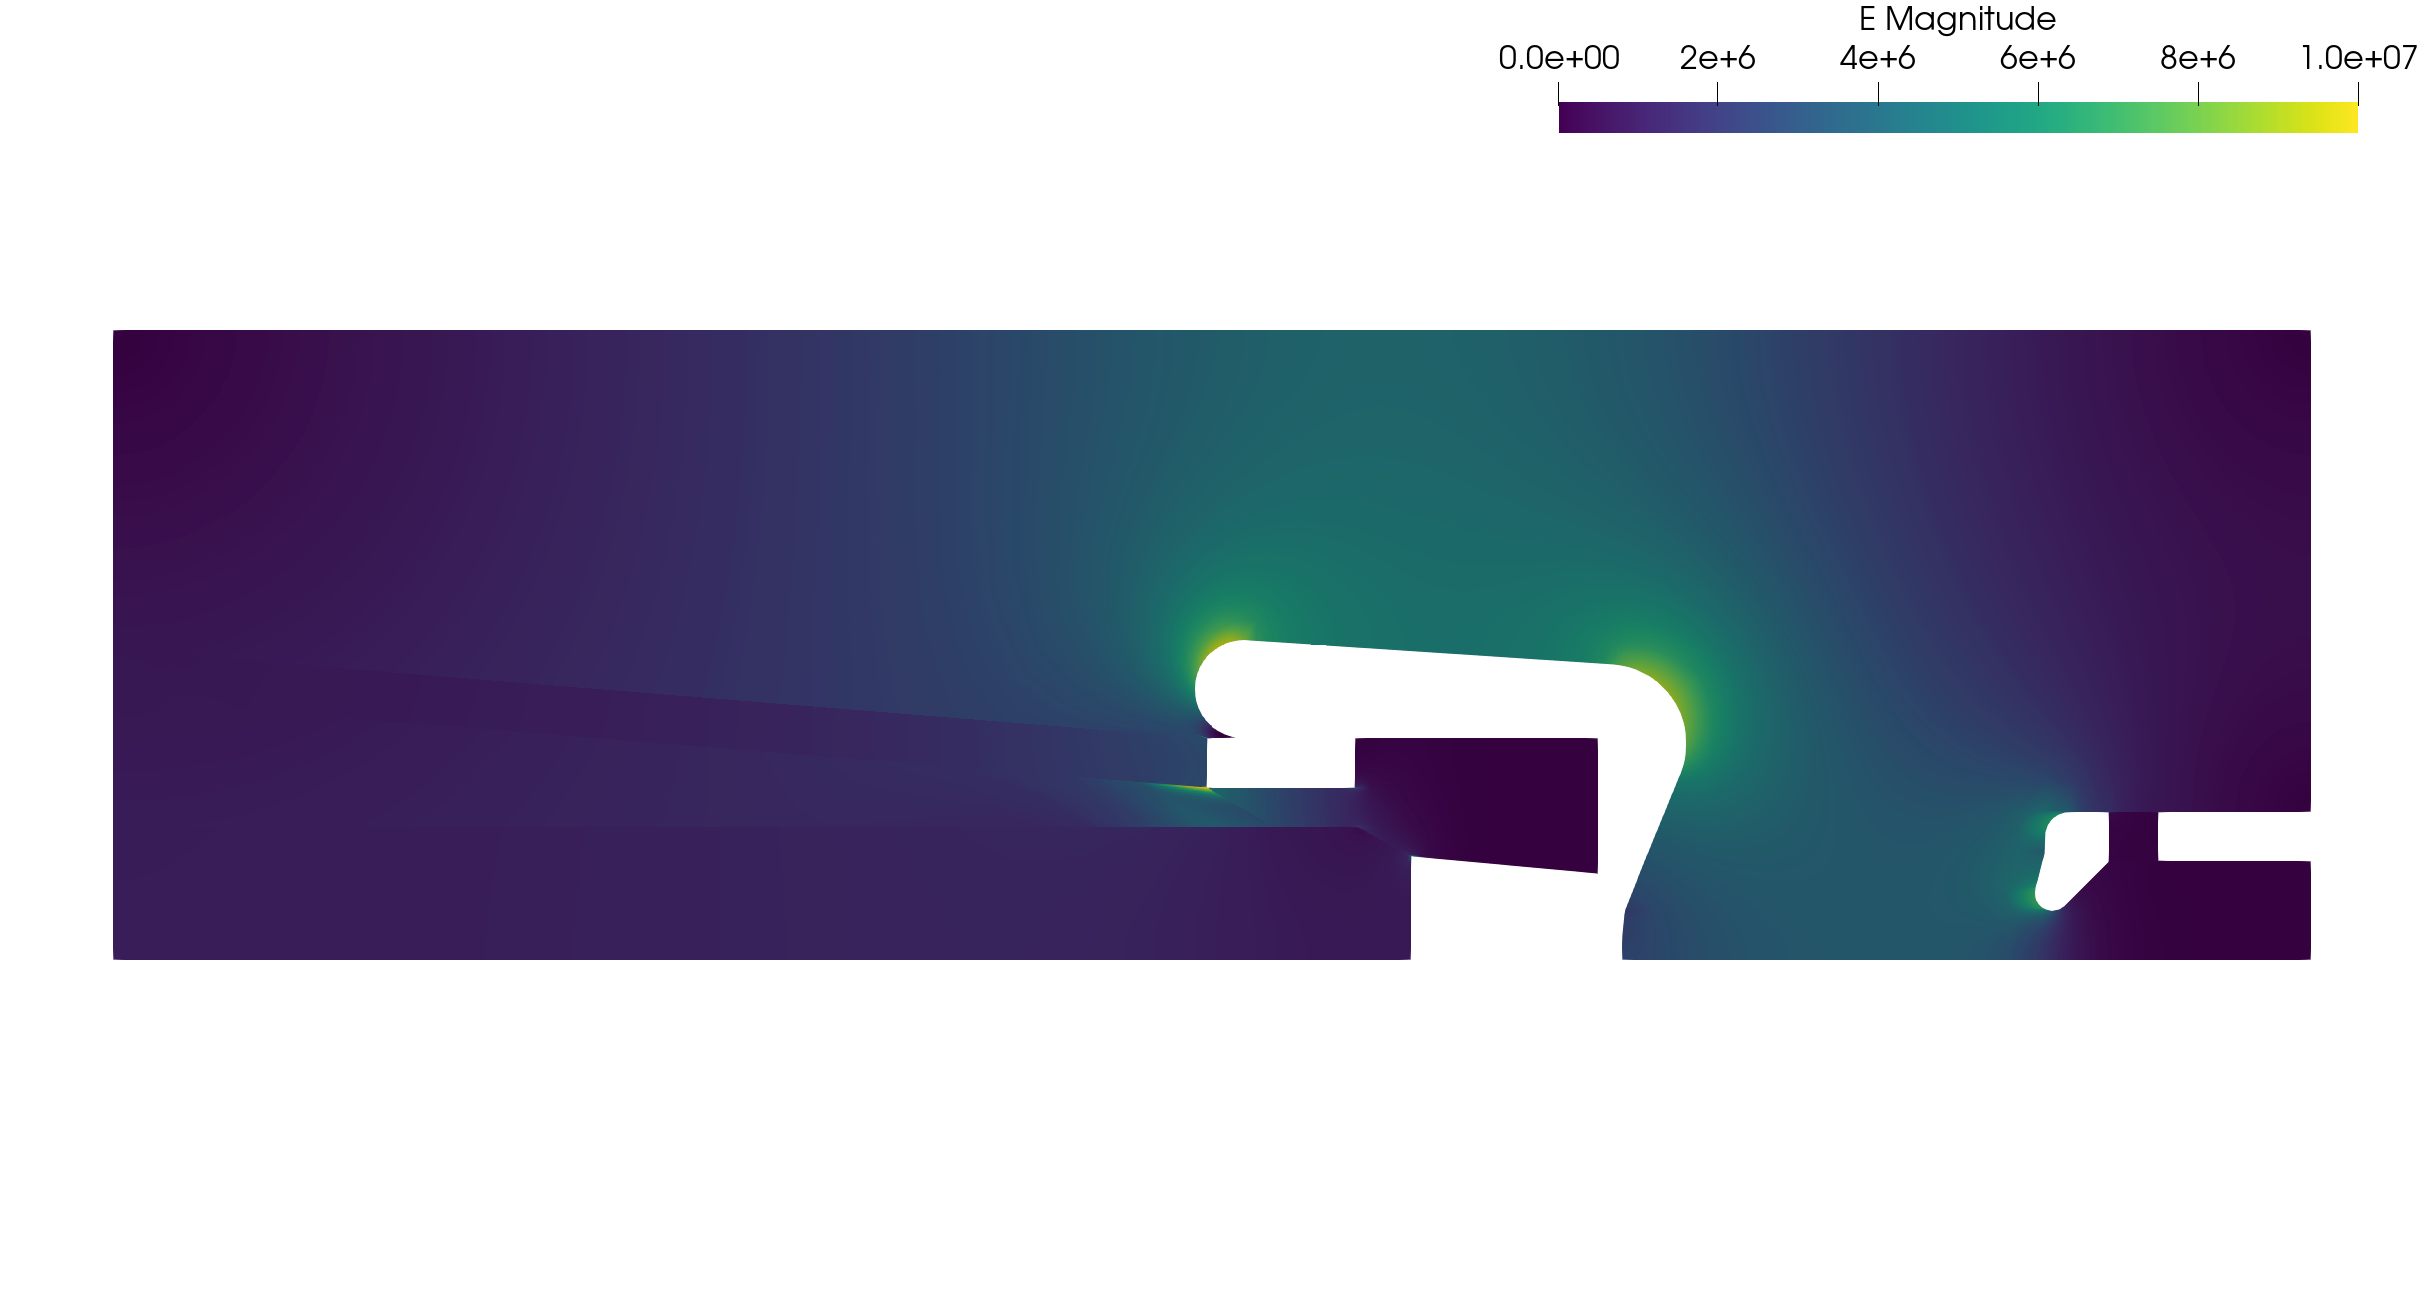
\includegraphics[width=\textwidth]{fig/E_v6}
   \end{subfigure}
   \caption{Initial geometry and magnitude of electric field.}
   \label{fig:init}
\end{figure}
\end{center}

\subsection{Optimization}
\begin{itemize}
   \item optimized geometry in Figure \ref{fig:opt}
   \item cost function only takes into account electric field
   \item only the upper electrode shape is optimized (volume constraint could be kept as before at $625\ \mathrm{cm}^3$)
   \item corresponding electric field for $p=3$, $n_\mathrm{sub}=16$,  $V_\mathrm{el}=-300\ \mathrm{kV}$ and $V_\mathrm{ar}=1\ \mathrm{kV}$
   \item \textbf{magnitude of E-field remains large in patch 14} (also around anode ring)
   \item \textbf{results}: \qquad
                           \begin{tabular}{c|c|c}
                              & $(V_\mathrm{el}-625) / \mathrm{cm}^3$ & $\max(\mathbf{\|E\|_2}) / \frac{\mathrm{MV}}{\mathrm{m}}$ \\
                              \hline
                              initial & 2.445 & 9.295 \\
                              optimized & -12.872 & 8.49 \\
                            \end{tabular}
\end{itemize}

\begin{center}
\begin{figure}[H]
   \begin{subfigure}{0.45\textwidth}
      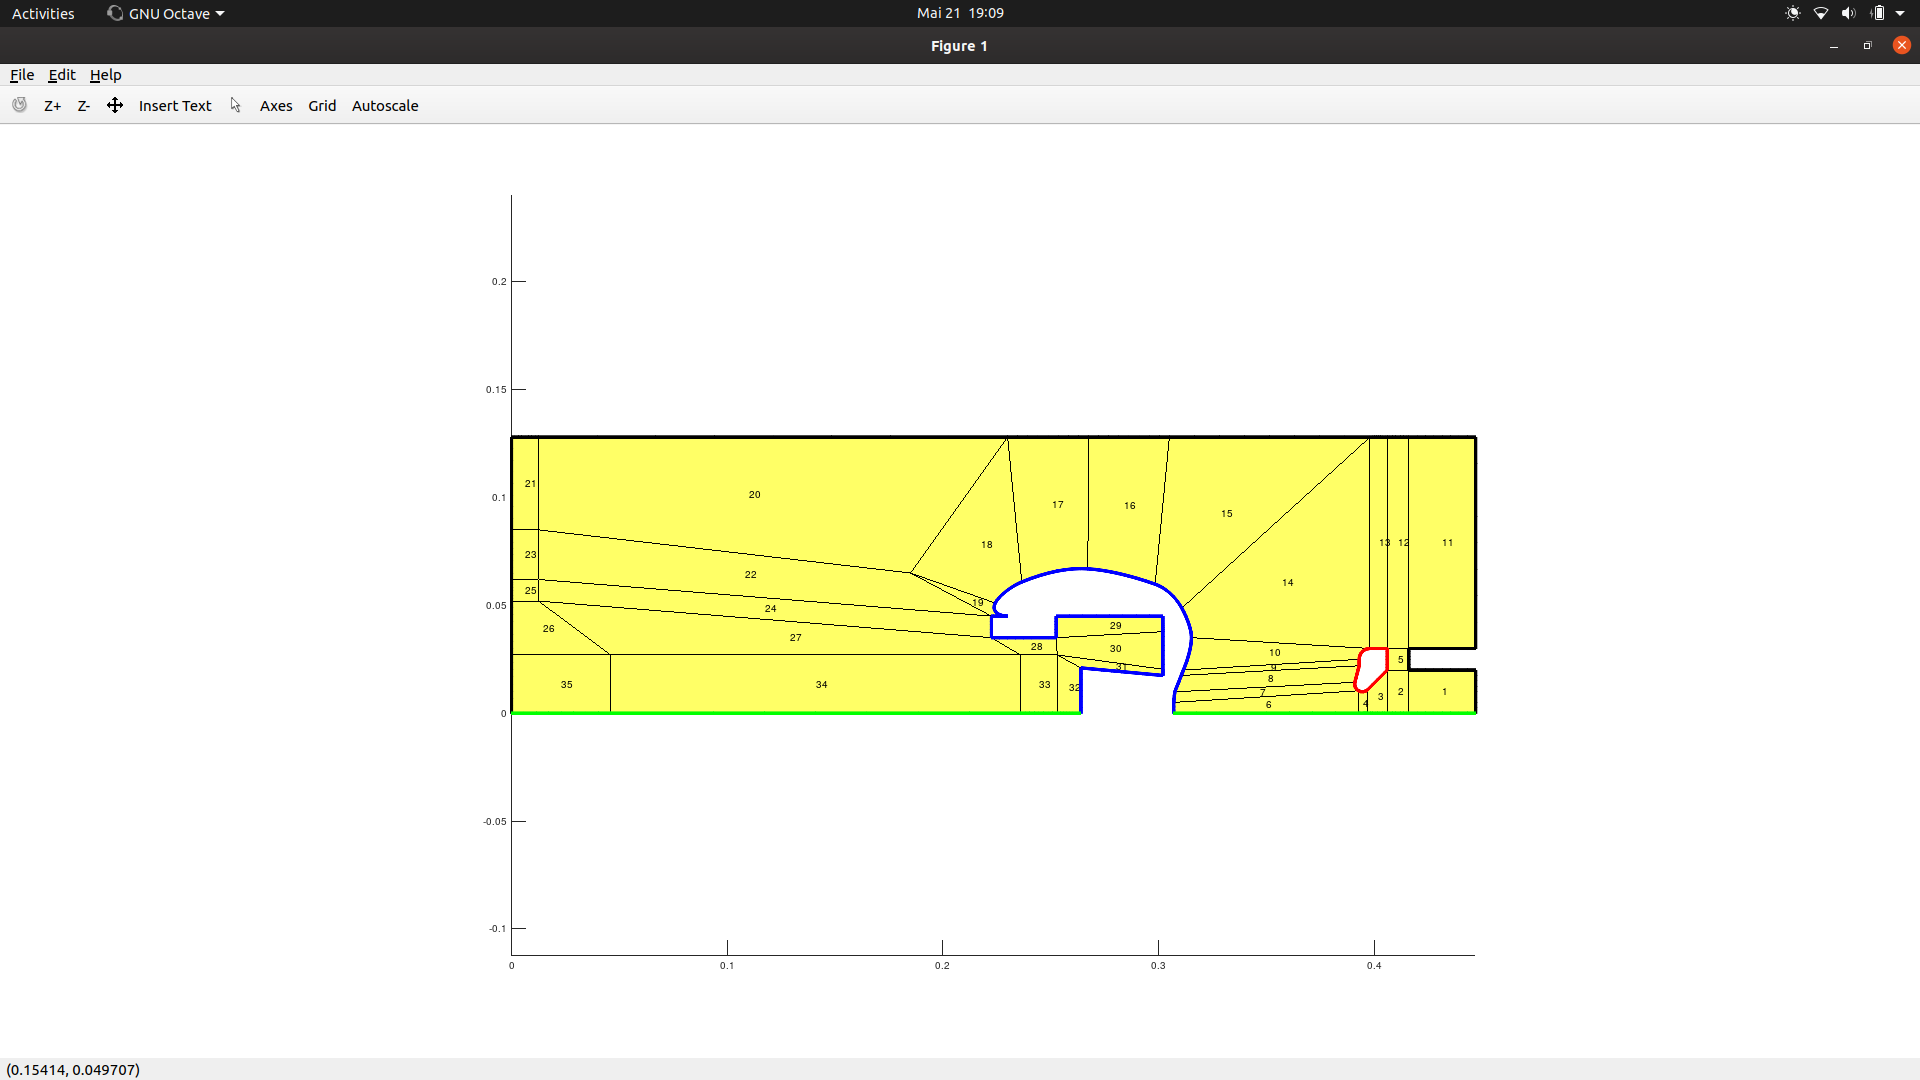
\includegraphics[width=\textwidth]{fig/geometry_v6_opt_order=3_run2}
   \end{subfigure}
   \begin{subfigure}{0.45\textwidth}
      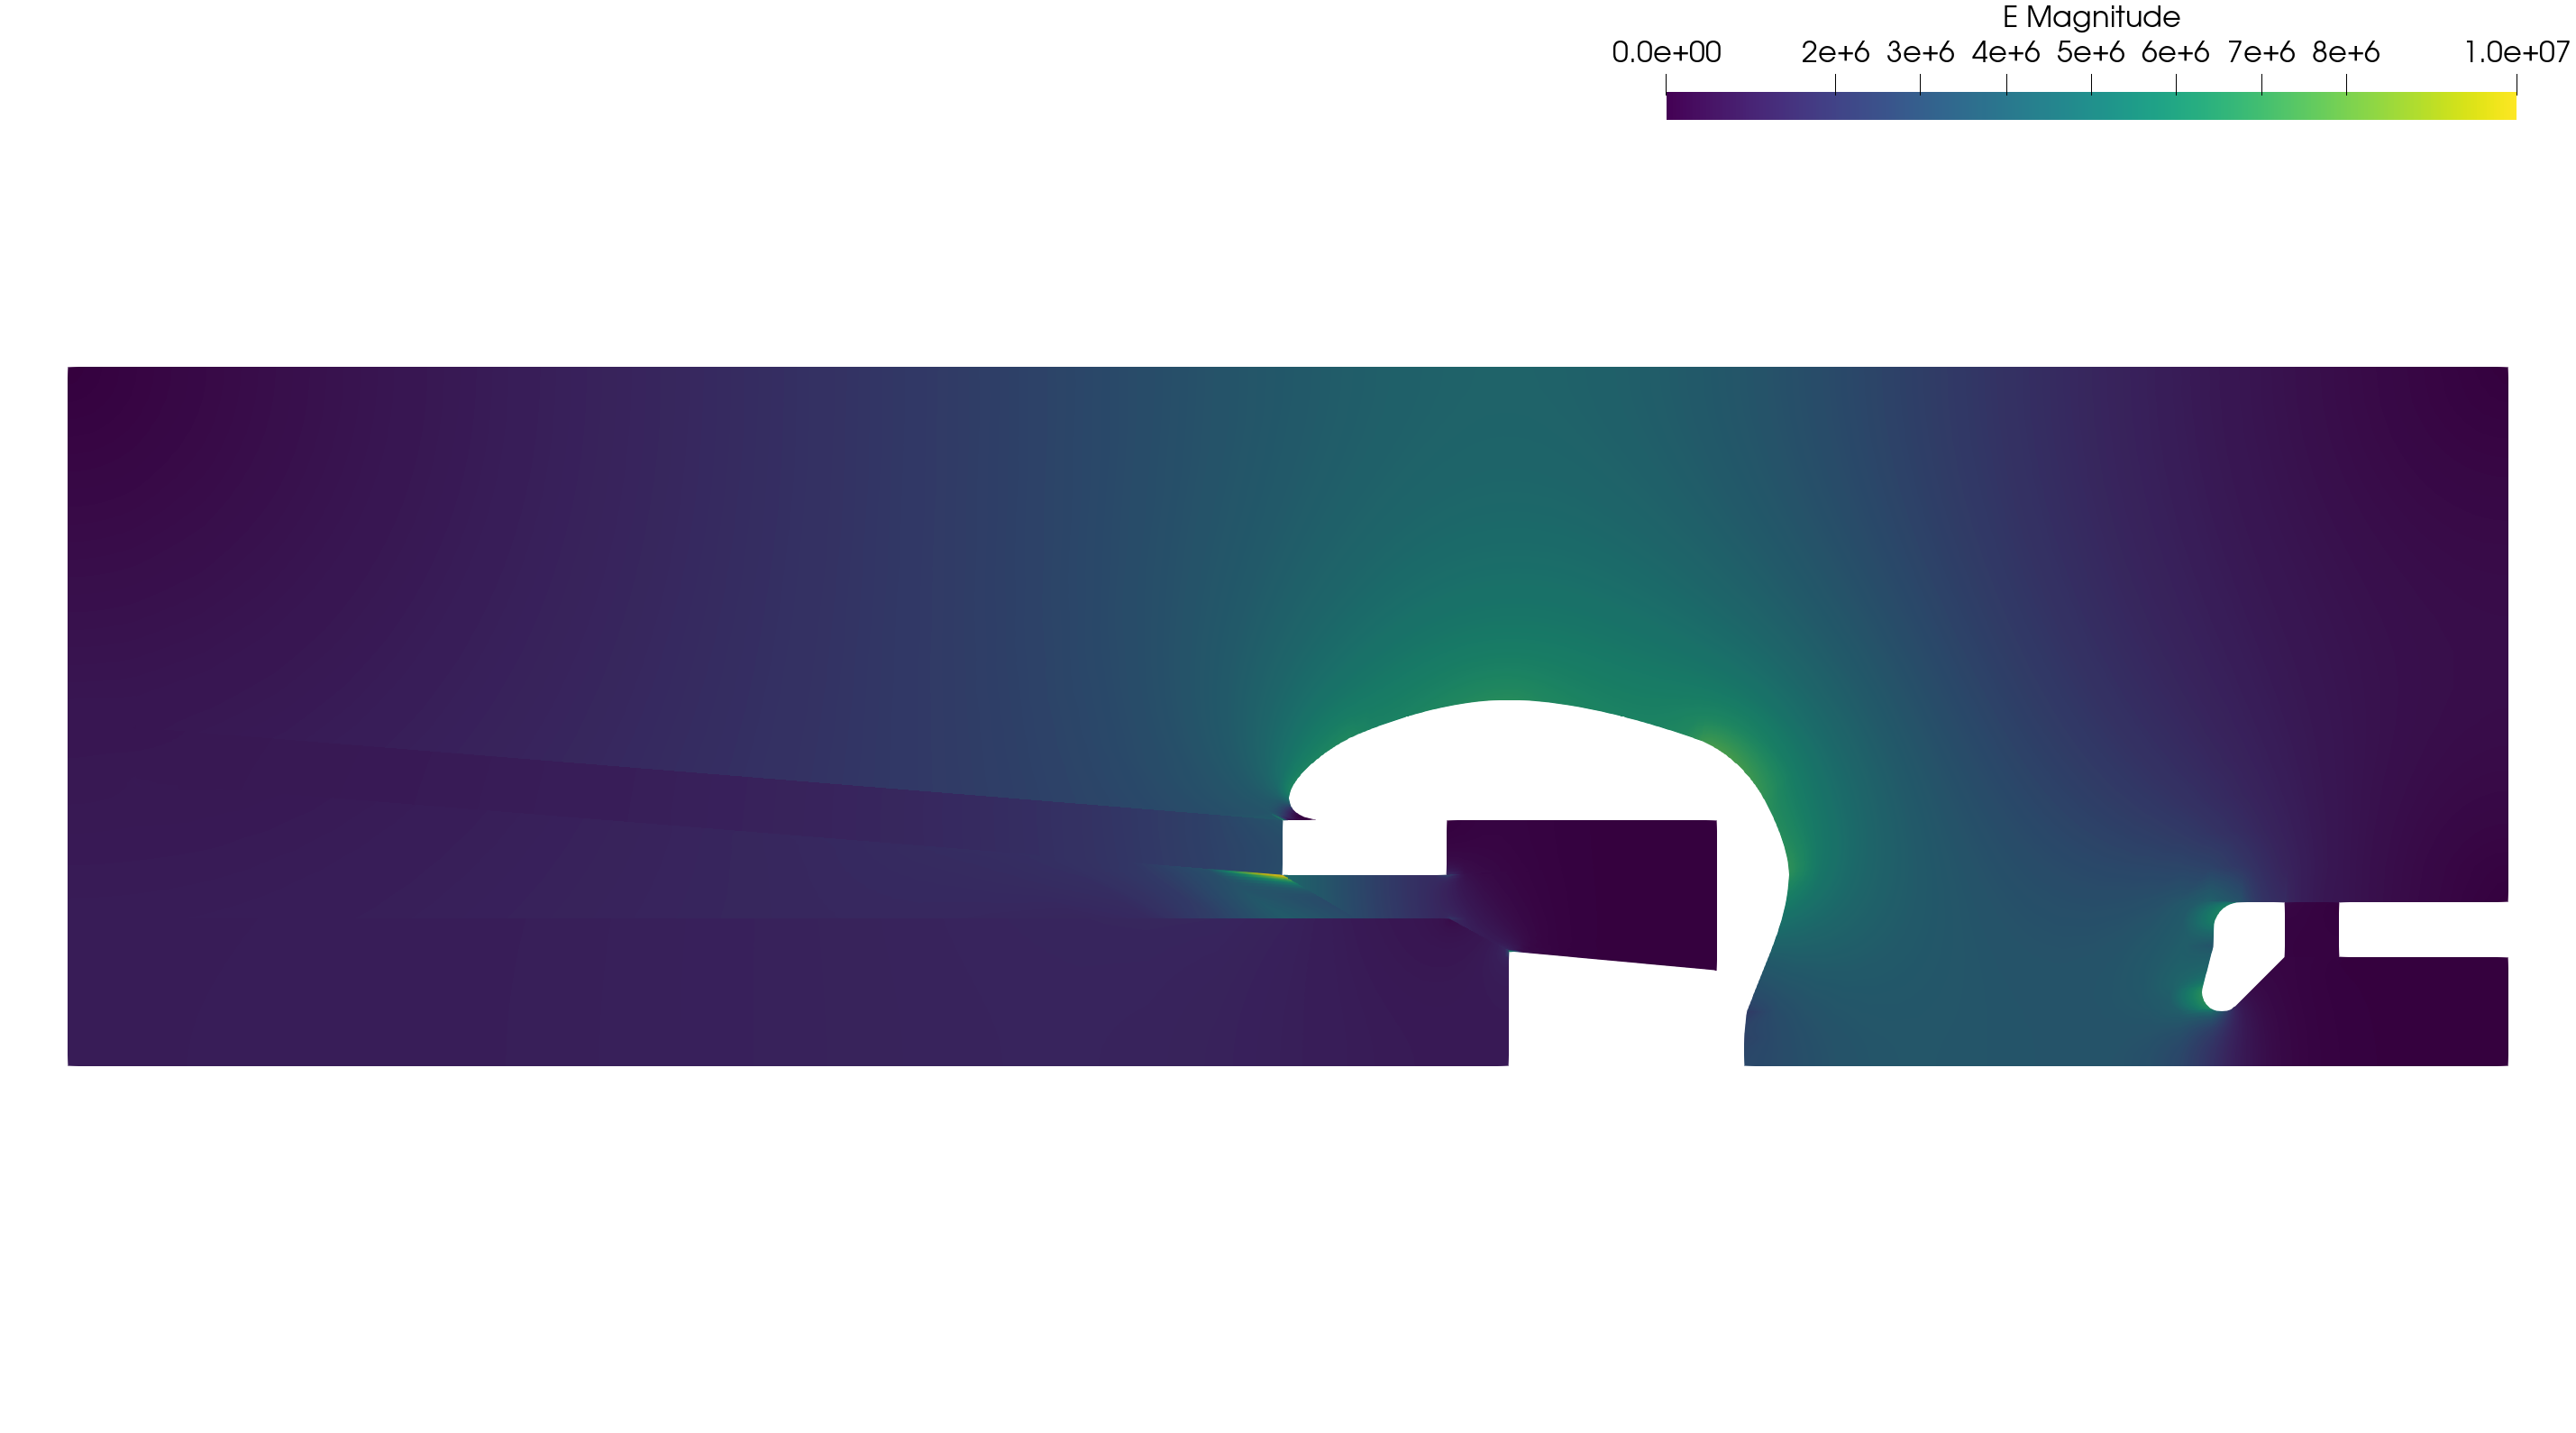
\includegraphics[width=\textwidth]{fig/E_v6_opt_order=3_run2}
   \end{subfigure}
   \caption{Optimized geometry and electric field.}
   \label{fig:opt}
\end{figure}
\end{center}

\subsection{Tracking}
\begin{itemize}
   \item \textbf{general settings}: $Q=100\ \mathrm{fC}$
   \item \textbf{spatial distribution}: Gaussian with $\sigma=400\ \mu\mathrm{m}$, see Figure \ref{fig:gen_sp} for comparison with laser measurement (probe particles at $0.5\sigma$, $\sigma$, $1.5\sigma$ in red)
   \item \textbf{temporal distribution}: Gaussian with $\sigma=5\ \mathrm{ps}$, see Figure \ref{fig:gen_tmp} for comparison with measurement/model from \cite{wagner}
\end{itemize}

\begin{center}
\begin{figure}[H]
   \begin{subfigure}{0.4\textwidth}
      \begin{tikzpicture}
   \begin{axis}[
      axis equal,
      try min ticks=6,
      max space between ticks=1000pt,
      enlargelimits=true,
      xlabel=$x\ \mathrm{in}\ \mathrm{mm}$,
      ylabel=$y\ \mathrm{in}\ \mathrm{mm}$,
      ]

      \addplot[color=TUDa-1a, only marks, mark=*] table {fig/astra/gen/I=1024_Q=0.0001_sc=0.005_gen.dat};
      \addplot[color=TUDa-1a, only marks, mark=*] table {fig/astra/gen/I=1024_Q=0.0001_sc=0.005_probe.dat};
      % \addplot[color=TUDa-9a, only marks, mark=*] table {fig/astra/gen/laser_I=1024_Q=0.0001_sc=0.005_probe.dat};

   \end{axis}
\end{tikzpicture}

   \end{subfigure}
   \qquad \qquad \qquad
   \begin{subfigure}{0.5\textwidth}
      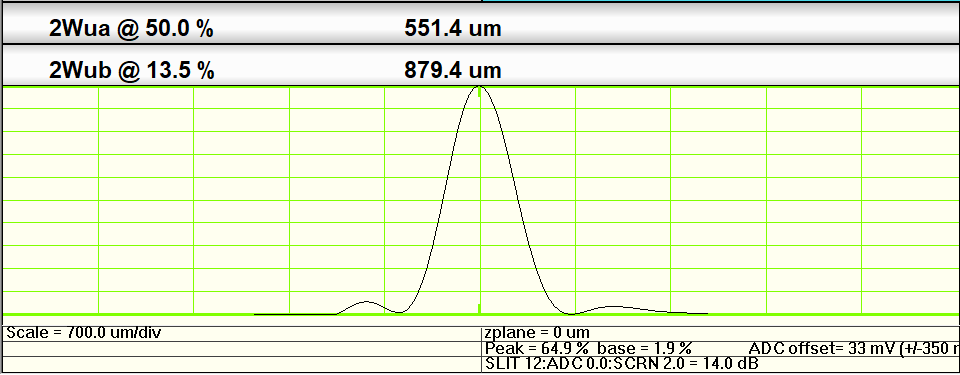
\includegraphics[width=\textwidth]{fig/laser}
   \end{subfigure}
   \caption{Spatial distribution ($2^{10}$ particles) and laser measurement.}
   \label{fig:gen_sp}
\end{figure}
\end{center}

\begin{center}
\begin{figure}[H]
   \begin{subfigure}{0.4\textwidth}
      \begin{tikzpicture}
   \begin{axis}[
      try min ticks=6,
      max space between ticks=1000pt,
      enlargelimits=true,
      xlabel=$t\ \mathrm{in\ ps}$,
      ylabel=$N_\mathrm{part}$,
      ]

      \addplot[color=TUDa-1a, ultra thick] table {fig/astra/gen/laser_I=2048_Q=0.0001_sc=0.005_tmp.dat};

   \end{axis}
\end{tikzpicture}

   \end{subfigure}
   \qquad \qquad \qquad
   \begin{subfigure}{0.5\textwidth}
      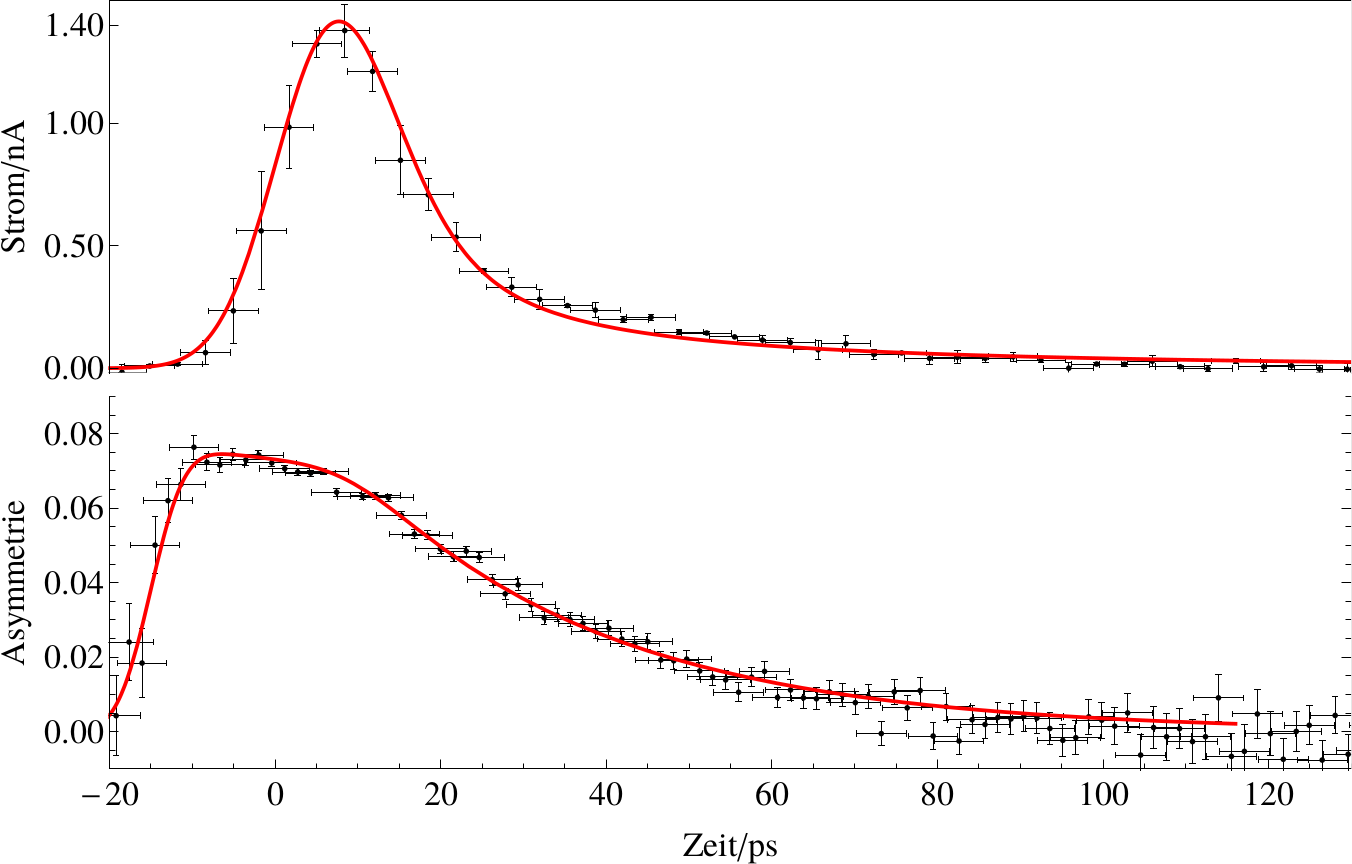
\includegraphics[width=\textwidth]{fig/bunch}
   \end{subfigure}
   \caption{Temporal distribution ($2^{10}$ particles) and measurement/model.}
   \label{fig:gen_tmp}
\end{figure}
\end{center}

% \newpage
%
% \begin{itemize}
%    \item \textbf{convergence of time integrator}: difference of normalized transverse emmitance $\epsilon$ w.\,r.\,t.\ finest time step is shown in Figure \ref{fig:int_cvg}
%    \item $H=2^{-11}\ \mathrm{ns}$ used later on
% \end{itemize}
%
% \begin{center}
% \begin{figure}[H]
%    \begin{subfigure}{0.4\textwidth}
%       \begin{tikzpicture}
   \begin{axis}[
      axis equal,
      try min ticks=4,
      max space between ticks=1000pt,
      enlargelimits=true,
      xlabel=$z / \mathrm{m}$,
      ylabel=$\epsilon / \mathrm{mrad\ mm}$,
      ]

      \addplot[color=TUDa-1a] table {fig/astra/int/photogun_int_emit_H_it=-13.dat};
      \addlegendentry{$H=2^{-13}$}
      \addplot[color=TUDa-2a] table {fig/astra/int/photogun_int_emit_H_it=-12.dat};
      \addlegendentry{$H=2^{-12}$}
      \addplot[color=TUDa-3a] table {fig/astra/int/photogun_int_emit_H_it=-11.dat};
      \addlegendentry{$H=2^{-11}$}
      \addplot[color=TUDa-4a] table {fig/astra/int/photogun_int_emit_H_it=-10.dat};
      \addlegendentry{$H=2^{-10}$}
      \addplot[color=TUDa-5a] table {fig/astra/int/photogun_int_emit_H_it=-9.dat};
      \addlegendentry{$H=2^{-9}$}
      \addplot[color=TUDa-6a] table {fig/astra/int/photogun_int_emit_H_it=-8.dat};
      \addlegendentry{$H=2^{-8}$}

   \end{axis}
\end{tikzpicture}

%    \end{subfigure}
%    \qquad \qquad \qquad
%    \begin{subfigure}{0.4\textwidth}
%       \begin{tikzpicture}
   \begin{loglogaxis}[
      axis equal,
      try min ticks=4,
      max space between ticks=1000pt,
      enlargelimits=true,
      xlabel=$H / \mathrm{ns}$,
      ylabel=$\|\Delta \epsilon\|_\infty / \mathrm{mrad\ mm}$,
      ]

      \addplot[color=TUDa-1a, ultra thick] table {fig/astra/int/photogun_int_err.dat};

   \end{loglogaxis}
\end{tikzpicture}

%    \end{subfigure}
%    \caption{Normalized transverse emmitance and absolute error in $l_\infty$-norm.}
%    \label{fig:int_cvg}
% \end{figure}
% \end{center}
%
% \begin{itemize}
%    \item \textbf{convergence of field map}: look at convergence with number of grid points in transverse $(n_x, n_y)$ and longitudinal $(n_z)$ direction individually
%    \item Figure \ref{fig:map_cvg_xy} looks at convergence of $n_x, n_y$ for $n_z=64$
%    \item Figure \ref{fig:map_cvg_z} looks at convergence of $n_z$ for $n_x=n_y=16$
%    \item $n_x=n_y=16$ and $n_z=64$ used later on
% \end{itemize}
%
% \begin{center}
% \begin{figure}[H]
%    \begin{subfigure}{0.4\textwidth}
%       \begin{tikzpicture}
   \begin{axis}[
      axis equal,
      try min ticks=4,
      max space between ticks=1000pt,
      enlargelimits=true,
      xlabel=$z / \mathrm{m}$,
      ylabel=$\epsilon / \mathrm{mrad\ mm}$,
      ]

      \addplot[color=TUDa-1a] table {fig/astra/map/photogun_map_emit_nx=ny=8_nz=64.dat};
      \addlegendentry{$n_x=8$}
      \addplot[color=TUDa-2a] table {fig/astra/map/photogun_map_emit_nx=ny=16_nz=64.dat};
      \addlegendentry{$n_x=16$}
      \addplot[color=TUDa-3a] table {fig/astra/map/photogun_map_emit_nx=ny=32_nz=64.dat};
      \addlegendentry{$n_x=32$}
      \addplot[color=TUDa-4a] table {fig/astra/map/photogun_map_emit_ref_nx=ny=64_nz=64.dat};
      \addlegendentry{$n_x=64$}

   \end{axis}
\end{tikzpicture}

%    \end{subfigure}
%    \qquad \qquad \qquad
%    \begin{subfigure}{0.4\textwidth}
%       \begin{tikzpicture}
   \begin{loglogaxis}[
      axis equal,
      try min ticks=4,
      max space between ticks=1000pt,
      enlargelimits=true,
      xlabel=$n_x$,
      ylabel=$\|\Delta \epsilon\|_\infty / \mathrm{mrad\ mm}$,
      ]

      \addplot[color=TUDa-1a, ultra thick] table {fig/astra/map/photogun_map_err_nz=64.dat};

   \end{loglogaxis}
\end{tikzpicture}

%    \end{subfigure}
%    \caption{Normalized transverse emmitance and absolute error in $l_\infty$-norm for $n_z=64$ and $n_x=n_y$ variable.}
%    \label{fig:map_cvg_xy}
% \end{figure}
% \end{center}
%
% \begin{center}
% \begin{figure}[H]
%    \begin{subfigure}{0.4\textwidth}
%       \begin{tikzpicture}
   \begin{axis}[
      axis equal,
      try min ticks=4,
      max space between ticks=1000pt,
      enlargelimits=true,
      xlabel=$z\ \mathrm{in\ m}$,
      ylabel=$\epsilon\ \mathrm{in\ mrad\ mm}$,
      ]

      \addplot[color=TUDa-1a] table {fig/astra/map/nz/photogun_map_emit_nx=ny=8_nz=16.dat};
      \addlegendentry{$n_z=16$}
      \addplot[color=TUDa-2a] table {fig/astra/map/nz/photogun_map_emit_nx=ny=8_nz=32.dat};
      \addlegendentry{$n_x=32$}
      \addplot[color=TUDa-3a] table {fig/astra/map/nz/photogun_map_emit_nx=ny=8_nz=64.dat};
      \addlegendentry{$n_x=64$}
      \addplot[color=TUDa-4a] table {fig/astra/map/nz/photogun_map_emit_nx=ny=8_nz=128.dat};
      \addlegendentry{$n_x=128$}
      \addplot[color=TUDa-5a] table {fig/astra/map/nz/photogun_map_emit_nx=ny=8_nz=256.dat};
      \addlegendentry{$n_x=256$}
      \addplot[color=TUDa-6a] table {fig/astra/map/nz/photogun_map_emit_ref_nx=ny=8_nz=512.dat};
      \addlegendentry{$n_x=512$}

   \end{axis}
\end{tikzpicture}

%    \end{subfigure}
%    \qquad \qquad \qquad
%    \begin{subfigure}{0.4\textwidth}
%       \begin{tikzpicture}
   \begin{loglogaxis}[
      try min ticks=4,
      max space between ticks=1000pt,
      enlargelimits=true,
      xlabel=$h_z\ \mathrm{in\ m}$,
      ylabel=$\mathrm{relative\ error\ in}\ l_\infty \mathrm{-norm}$,
      ]

      \addplot[color=TUDa-1a, ultra thick, mark=*] table {fig/astra/map/nz/photogun_map_err_nx=ny=8.dat};

   \end{loglogaxis}
\end{tikzpicture}

%    \end{subfigure}
%    \caption{Normalized transverse emmitance and absolute error in $l_\infty$-norm for $n_z$ variable and $n_x=n_y=16$.}
%    \label{fig:map_cvg_z}
% \end{figure}
% \end{center}
%
% \begin{itemize}
%    \item \textbf{convergence of space charge}: look at convergence with number of grid cells in radial $(n_r)$ and longitudinal $(n_l)$ direction and number of particles $(n_I)$ separately
%
%    \item Figure \ref{fig:sc_cvg_rl} looks at convergence of $n_r, n_l$ for $n_I=2^{10}$
%    \item $n_r=n_l=16$ used later on
%
%    \item Figure \ref{fig:sc_cvg_I} looks at convergence of $n_I$ for $n_r=n_l=16$
%    \item $n_I=2^{10}$
% \end{itemize}
%
% \begin{center}
% \begin{figure}[H]
%    \begin{subfigure}{0.4\textwidth}
%       \begin{tikzpicture}
   \begin{axis}[
      axis equal,
      try min ticks=4,
      max space between ticks=1000pt,
      enlargelimits=true,
      xlabel=$z / \mathrm{m}$,
      ylabel=$\epsilon / \mathrm{mrad\ mm}$,
      legend style={fill=none}
      ]

      \addplot[color=TUDa-6a] table {fig/astra/sc/nr_nl/photogun_sc_emit_ref_nI=1024_nr=64_nc=2_nl=64.dat};
      \addlegendentry{$n_r=64\ n_l=64$}

      \addplot[color=TUDa-5a] table {fig/astra/sc/nr_nl/photogun_sc_emit_ref_nI=1024_nr=32_nc=2_nl=32.dat};
      \addlegendentry{$n_r=32\ n_l=32$}

      \addplot[color=TUDa-1a] table {fig/astra/sc/nr_nl/photogun_sc_emit_nI=1024_nr=4_nc=2_nl=4.dat};
      % \addlegendentry{$n_r=4\ n_l=4$}
      \addplot[color=TUDa-1a, dotted] table {fig/astra/sc/nr_nl/photogun_sc_emit_nI=1024_nr=4_nc=2_nl=8.dat};
      % \addlegendentry{$n_r=4\ n_l=8$}
      \addplot[color=TUDa-1a, dashed] table {fig/astra/sc/nr_nl/photogun_sc_emit_nI=1024_nr=4_nc=2_nl=16.dat};
      % \addlegendentry{$n_r=4\ n_l=16$}
      \addplot[color=TUDa-1a, dashdotted] table {fig/astra/sc/nr_nl/photogun_sc_emit_nI=1024_nr=4_nc=2_nl=32.dat};
      % \addlegendentry{$n_r=4\ n_l=32$}

      \addplot[color=TUDa-2a] table {fig/astra/sc/nr_nl/photogun_sc_emit_nI=1024_nr=8_nc=2_nl=4.dat};
      % \addlegendentry{$n_r=8\ n_l=4$}
      \addplot[color=TUDa-2a, dotted] table {fig/astra/sc/nr_nl/photogun_sc_emit_nI=1024_nr=8_nc=2_nl=8.dat};
      % \addlegendentry{$n_r=8\ n_l=8$}
      \addplot[color=TUDa-2a, dashed] table {fig/astra/sc/nr_nl/photogun_sc_emit_nI=1024_nr=8_nc=2_nl=16.dat};
      % \addlegendentry{$n_r=8\ n_l=16$}
      \addplot[color=TUDa-2a, dashdotted] table {fig/astra/sc/nr_nl/photogun_sc_emit_nI=1024_nr=8_nc=2_nl=32.dat};
      % \addlegendentry{$n_r=8\ n_l=32$}

      \addplot[color=TUDa-3a] table {fig/astra/sc/nr_nl/photogun_sc_emit_nI=1024_nr=16_nc=2_nl=4.dat};
      % \addlegendentry{$n_r=16\ n_l=4$}
      \addplot[color=TUDa-3a, dotted] table {fig/astra/sc/nr_nl/photogun_sc_emit_nI=1024_nr=16_nc=2_nl=8.dat};
      % \addlegendentry{$n_r=16\ n_l=8$}
      \addplot[color=TUDa-3a, dashed] table {fig/astra/sc/nr_nl/photogun_sc_emit_nI=1024_nr=16_nc=2_nl=16.dat};
      % \addlegendentry{$n_r=16\ n_l=16$}
      \addplot[color=TUDa-3a, dashdotted] table {fig/astra/sc/nr_nl/photogun_sc_emit_nI=1024_nr=16_nc=2_nl=32.dat};
      % \addlegendentry{$n_r=16\ n_l=32$}

      \addplot[color=TUDa-4a] table {fig/astra/sc/nr_nl/photogun_sc_emit_nI=1024_nr=32_nc=2_nl=4.dat};
      % \addlegendentry{$n_r=32\ n_l=4$}
      \addplot[color=TUDa-4a, dotted] table {fig/astra/sc/nr_nl/photogun_sc_emit_nI=1024_nr=32_nc=2_nl=8.dat};
      % \addlegendentry{$n_r=32\ n_l=8$}
      \addplot[color=TUDa-4a, dashed] table {fig/astra/sc/nr_nl/photogun_sc_emit_nI=1024_nr=32_nc=2_nl=16.dat};
      % \addlegendentry{$n_r=32\ n_l=16$}

   \end{axis}
\end{tikzpicture}

%    \end{subfigure}
%    \qquad \qquad \qquad
%    \begin{subfigure}{0.4\textwidth}
%       \begin{tikzpicture}
   \begin{loglogaxis}[
      try min ticks=4,
      max space between ticks=1000pt,
      enlargelimits=true,
      xlabel=$n_l$,
      ylabel=$\|\Delta \epsilon\|_\infty / \mathrm{mrad\ mm}$,
      ]

      \addplot[color=TUDa-1a, ultra thick] table {fig/astra/sc/nr_nl/photogun_sc_err_nI=1024_nr=4_nc=2.dat};
      \addlegendentry{$n_r=4$}
      \addplot[color=TUDa-2a, ultra thick] table {fig/astra/sc/nr_nl/photogun_sc_err_nI=1024_nr=8_nc=2.dat};
      \addlegendentry{$n_r=8$}
      \addplot[color=TUDa-3a, ultra thick] table {fig/astra/sc/nr_nl/photogun_sc_err_nI=1024_nr=16_nc=2.dat};
      \addlegendentry{$n_r=16$}
      \addplot[color=TUDa-4a, ultra thick] table {fig/astra/sc/nr_nl/photogun_sc_err_nI=1024_nr=32_nc=2.dat};
      \addlegendentry{$n_r=32$}

   \end{loglogaxis}
\end{tikzpicture}

%    \end{subfigure}
%    \caption{Normalized transverse emmitance and absolute error in $l_\infty$-norm for $n_I=2^{10}$ and $n_l, n_r$ variable.}
%    \label{fig:sc_cvg_rl}
% \end{figure}
% \end{center}
%
% \begin{center}
% \begin{figure}[H]
%    \begin{subfigure}{0.4\textwidth}
%       \begin{tikzpicture}
   \begin{axis}[
      axis equal,
      try min ticks=4,
      max space between ticks=1000pt,
      enlargelimits=true,
      xlabel=$z / \mathrm{m}$,
      ylabel=$\epsilon / \mathrm{mrad\ mm}$,
      legend style={fill=none},
      legend pos=south east
      ]

      \addplot[color=TUDa-1a] table {fig/astra/sc/nI/photogun_sc_emit_nI=256_nr=16_nc=2_nl=16.dat};
      \addlegendentry{$n_I=2^{8}$}
      \addplot[color=TUDa-2a] table {fig/astra/sc/nI/photogun_sc_emit_nI=512_nr=16_nc=2_nl=16.dat};
      \addlegendentry{$n_I=2^{9}$}
      \addplot[color=TUDa-3a] table {fig/astra/sc/nI/photogun_sc_emit_nI=1024_nr=16_nc=2_nl=16.dat};
      \addlegendentry{$n_I=2^{10}$}
      \addplot[color=TUDa-4a] table {fig/astra/sc/nI/photogun_sc_emit_nI=2048_nr=16_nc=2_nl=16.dat};
      \addlegendentry{$n_I=2^{11}$}
      \addplot[color=TUDa-5a] table {fig/astra/sc/nI/photogun_sc_emit_nI=4096_nr=16_nc=2_nl=16.dat};
      \addlegendentry{$n_I=2^{12}$}

      \addplot[color=TUDa-6a] table {fig/astra/sc/nI/photogun_sc_emit_ref_nI=8192_nr=16_nc=2_nl=16.dat};
      \addlegendentry{$n_I=2^{13}$}

   \end{axis}
\end{tikzpicture}

%    \end{subfigure}
%    \qquad \qquad \qquad
%    \begin{subfigure}{0.4\textwidth}
%       \begin{tikzpicture}
   \begin{loglogaxis}[
      axis equal,
      try min ticks=4,
      max space between ticks=1000pt,
      enlargelimits=true,
      xlabel=$n_I$,
      ylabel=$\|\Delta \epsilon\|_\infty / \mathrm{mrad\ mm}$,
      ]

      \addplot[color=TUDa-1a, ultra thick] table {fig/astra/sc/nI/photogun_sc_err_nr=16_nc=2_nl=16.dat};

   \end{loglogaxis}
\end{tikzpicture}

%    \end{subfigure}
%    \caption{Normalized transverse emmitance and absolute error in $l_\infty$-norm for $n_I$ variable and $n_l=n_r=16$.}
%    \label{fig:sc_cvg_I}
% \end{figure}
% \end{center}

% Cell_var
% \begin{center}
% \begin{figure}[H]
%    \begin{subfigure}{0.4\textwidth}
%       \begin{tikzpicture}
   \begin{axis}[
      axis equal,
      try min ticks=4,
      max space between ticks=1000pt,
      enlargelimits=true,
      xlabel=$z / \mathrm{m}$,
      ylabel=$\epsilon / \mathrm{mrad\ mm}$,
      legend style={fill=none}
      ]

      \addplot[color=TUDa-1a] table {fig/astra/sc/nc/photogun_sc_emit_nI=1024_nr=16_nc=0.5_nl=16.dat};
      \addlegendentry{$n_c=0.5$}
      \addplot[color=TUDa-2a] table {fig/astra/sc/nc/photogun_sc_emit_nI=1024_nr=16_nc=2_nl=16.dat};
      \addlegendentry{$n_c=2$}
      \addplot[color=TUDa-3a] table {fig/astra/sc/nc/photogun_sc_emit_ref_nI=1024_nr=16_nc=4_nl=16.dat};
      \addlegendentry{$n_c=4$}

   \end{axis}
\end{tikzpicture}

%    \end{subfigure}
%    \qquad \qquad \qquad
%    \begin{subfigure}{0.4\textwidth}
%       \begin{tikzpicture}
   \begin{loglogaxis}[
      axis equal,
      try min ticks=4,
      max space between ticks=1000pt,
      enlargelimits=true,
      xlabel=$n_c$,
      ylabel=$\mathrm{relative\ error\ in}\ l_\infty \mathrm{-norm}$,
      ]

      \addplot[color=TUDa-1a, ultra thick, mark=*] table {fig/astra/sc/nc/photogun_sc_err_nI=1024_nr=64_nl=64.dat};

   \end{loglogaxis}
\end{tikzpicture}

%    \end{subfigure}
%    \caption{Normalized transversal emmitance and absolute error in $l_\infty$-norm for $n_I=2^{10}$ and $n_l=n_r=16$.}
%    \label{fig:sc_cvg_I}
% \end{figure}
% \end{center}

\begin{itemize}
   \item \textbf{tracking results}: $\epsilon$ and $x_\mathrm{rms}$ computed with the determined settings are shown in Figure \ref{fig:astra_res}
\end{itemize}

\begin{center}
\begin{figure}[H]
   \begin{subfigure}{0.4\textwidth}
      \begin{tikzpicture}
   \begin{axis}[
      axis equal,
      try min ticks=4,
      max space between ticks=1000pt,
      enlargelimits=true,
      xlabel=$z / \mathrm{m}$,
      ylabel=$\epsilon / \mathrm{mrad\ mm}$,
      legend style={fill=none}
      ]

      \addplot[color=TUDa-1a] table {fig/astra/results/photogun_init_eps.dat};
      \addlegendentry{initial}
      \addplot[color=TUDa-9a] table {fig/astra/results/photogun_run1_eps.dat};
      \addlegendentry{optimized}

   \end{axis}
\end{tikzpicture}

   \end{subfigure}
   \qquad \qquad \qquad
   \begin{subfigure}{0.4\textwidth}
      \begin{tikzpicture}
   \begin{axis}[
      try min ticks=4,
      max space between ticks=1000pt,
      enlargelimits=true,
      xlabel=$z / \mathrm{m}$,
      ylabel=$x_\mathrm{rms} / \mathrm{mm}$,
      legend style={fill=none}
      ]

      \addplot[color=TUDa-1a] table {fig/astra/results/photogun_init_rms.dat};
      \addlegendentry{initial}
      \addplot[color=TUDa-9a] table {fig/astra/results/photogun_run1_rms.dat};
      \addlegendentry{optimized}

   \end{axis}
\end{tikzpicture}

   \end{subfigure}
   \caption{Normalized transverse emmitance and rms beam size.}
   \label{fig:astra_res}
\end{figure}
\end{center}

\begin{itemize}
   \item \textbf{remarks}: the convergence studies also looked at $x_{rms}$ and the behavior was very similar to that of $\epsilon$\\

   \item to minimize the electric field on the entire electrode surface all curves could be taken into account
   \item this includes the anode ring shape, position and voltage
   \item also include tracking in optimization via $x_\mathrm{rms} \leq 1.5\ \mathrm{mm}$, also optimize or constrain $\epsilon \leq 1\ \mathrm{mrad\ mm}$?
\end{itemize}
